\documentclass[a4paper, 12pt]{article}
\usepackage[utf8]{inputenc}
\usepackage{geometry}
\usepackage{polski}
\usepackage{graphicx}
\usepackage{float}
\usepackage{etoolbox,refcount}
\usepackage{multicol}
\usepackage{tabularx}

\newgeometry{left=2cm, right=2cm, bottom=2cm, top=1.5cm}

\begin{document}
	\begin{figure}[H]
		\centering
		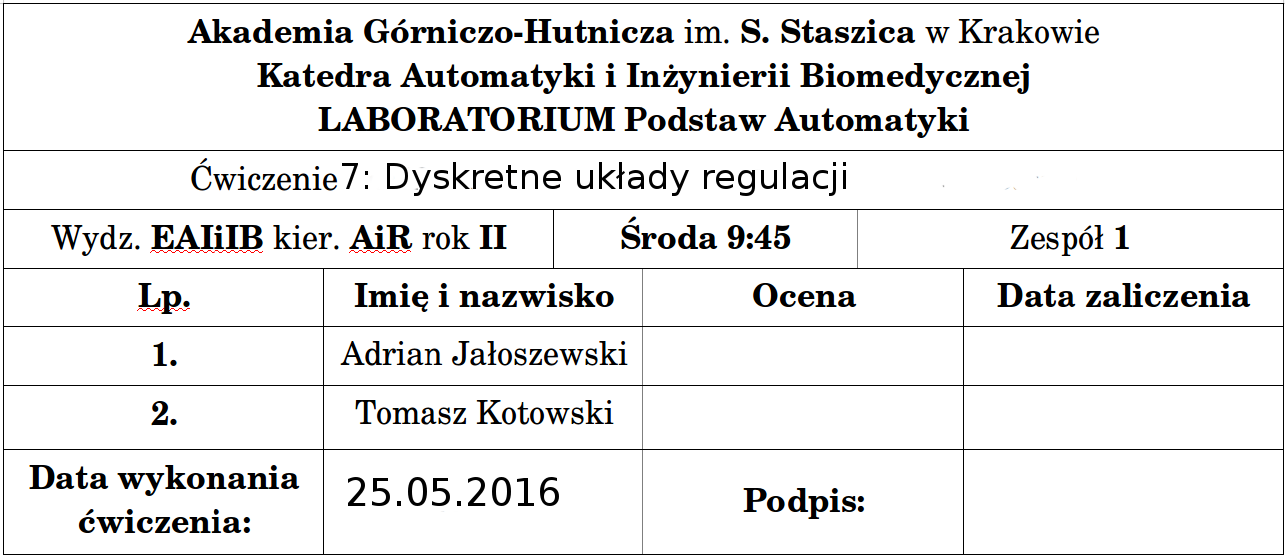
\includegraphics[width = \textwidth]{./img/cudo.png}
	\end{figure}
	\section{Cel ćwiczenia}
		Celem ćwiczenia jest zapoznanie się z podstawowymi własnościami układów regulacji składających się z ciągłego obiektu regulacji sterowanego regulatorem dyskretnym.
	\section{Wstęp}
		Pierwszy układ składał się z inercji I rzędu oraz regulatora P. Na wejście zadawany jest skok jednostkowy, a układ działa w sprzężeniu zwrotnym.
		\begin{figure}[H]
			\centering
			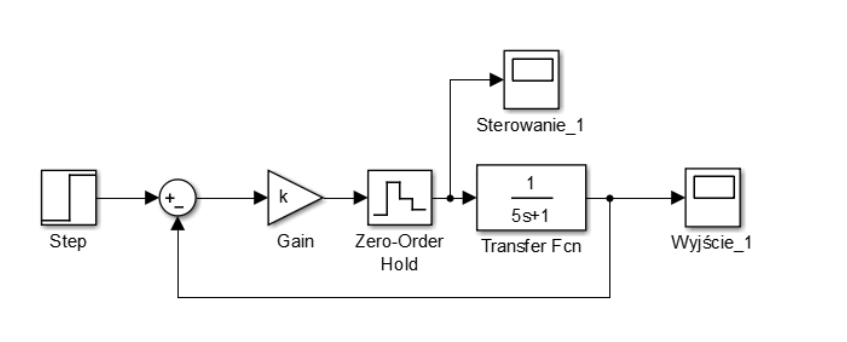
\includegraphics[width = \textwidth]{./img/uklad1.png}
			\caption{Inercja I rzędu}
		\end{figure}
		\noindent Jest to dyskretny układ regulacji z ekstrapolatorem zerowego rzędu. Oscyloskopy pobierają informacje o wyjściu z układu oraz o sterowaniu.
		\newline \newline
		Podobnym układem jest kolejny układ, w którym obiektem regulacji jest obiekt inercyjny III rzędu. Jeden oscyloskop odpowiada tu za wyświetlanie sterowania na wyjściu z regulatora,\linebreak a drugi za wyświetlanie przebiegów czasowych po każdej z inercji.
		\begin{figure}[H]
			\centering
			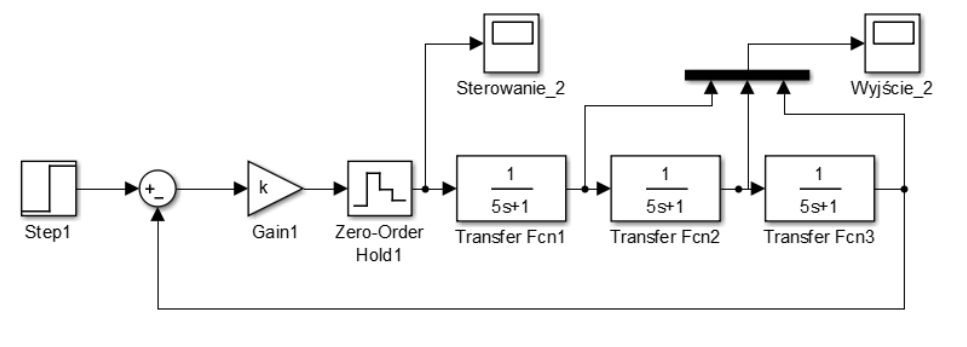
\includegraphics[width = \textwidth]{./img/uklad2.png}
			\caption{Inercja III rzędu}
		\end{figure}
		\noindent Dyskretne układy regulacji mogą stracić stabilność dla przypadków gdzie przy regulacji ciągłej układ zachowuje się stabilnie. Dobrym przykładem jest tu inercja pierwszego rzędu, która dla regulatora P jest układem strukturalnie stabilnym. Jest to układ strukturalnie stabilny, ponieważ jego charakterystyka amplitudowo--fazowa znajduje się zawsze w czwartej ćwiartce płaszczyzny zespolonej -- nigdy nie obejmuje punktu (-1, 0j).
		\begin{figure}[H]
			\centering
			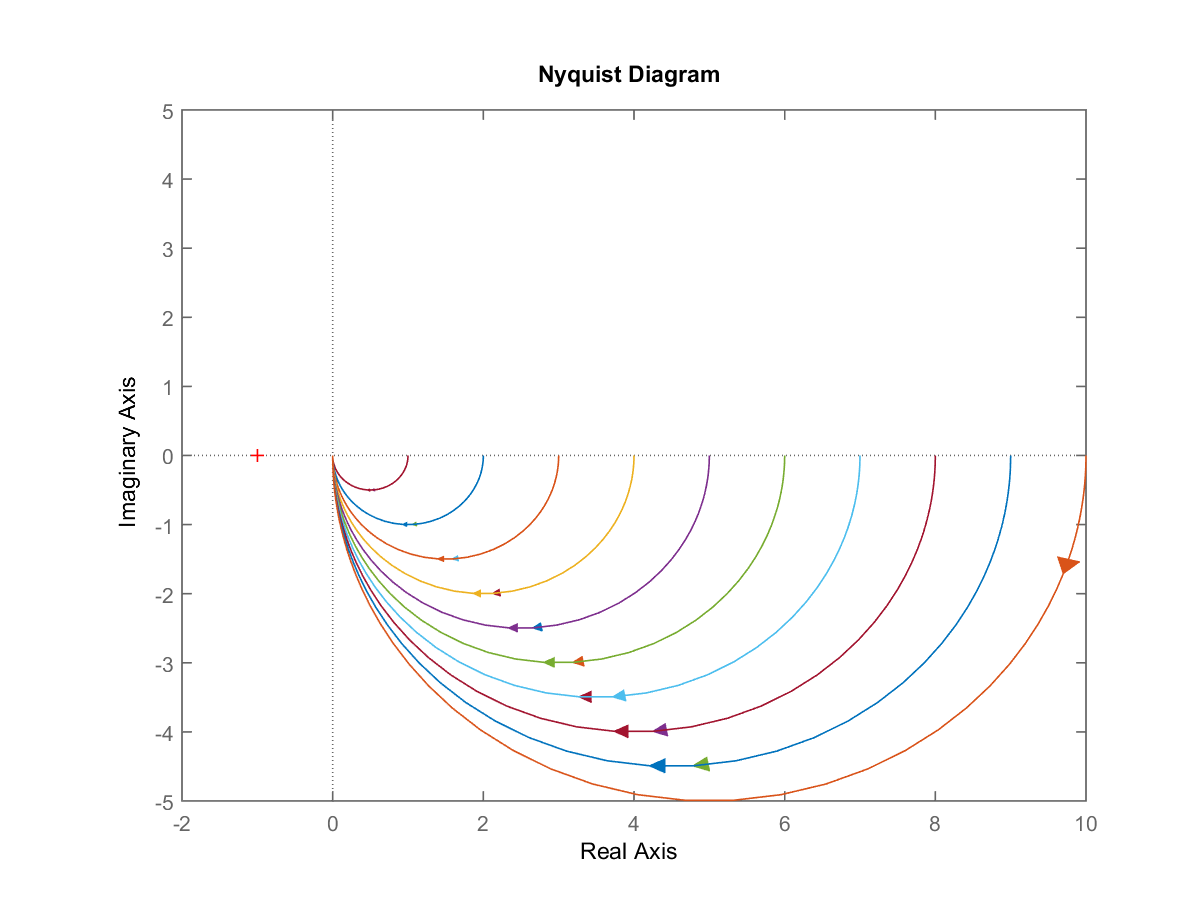
\includegraphics[width = \textwidth]{./img/uzasadnienie_jeden.png}
			\caption{Obiekty inercyjne I rzędu dla różnych parametrów.}
		\end{figure}
		\noindent Utrata stabilności w przypadku regulacji dyskretnej następuje na skutek tego, że transmitancja ekstrapolatora zerowego rzędu zawiera w sobie człon opóźniający.
	\section{Wyniki ćwiczenia}
		Wzmocnienia krytycznego szukaliśmy analizując to, czy przebieg jest tłumiony -- jeżeli tak, to zwiększaliśmy wzmocnienie, jeżeli nie, to obniżaliśmy je, dochodząc do chwili kiedy różnice były niezauważalnie małe.
		\subsection{Obiekt inercyjny I rzędu}
			Wyniki dla czasu próbkowania $T_p = 10 \, \mathrm{s}$. Wzmocnienie krytyczne: $k_{kr} = 1,3125$.
			\begin{figure}[H]
				\centering
				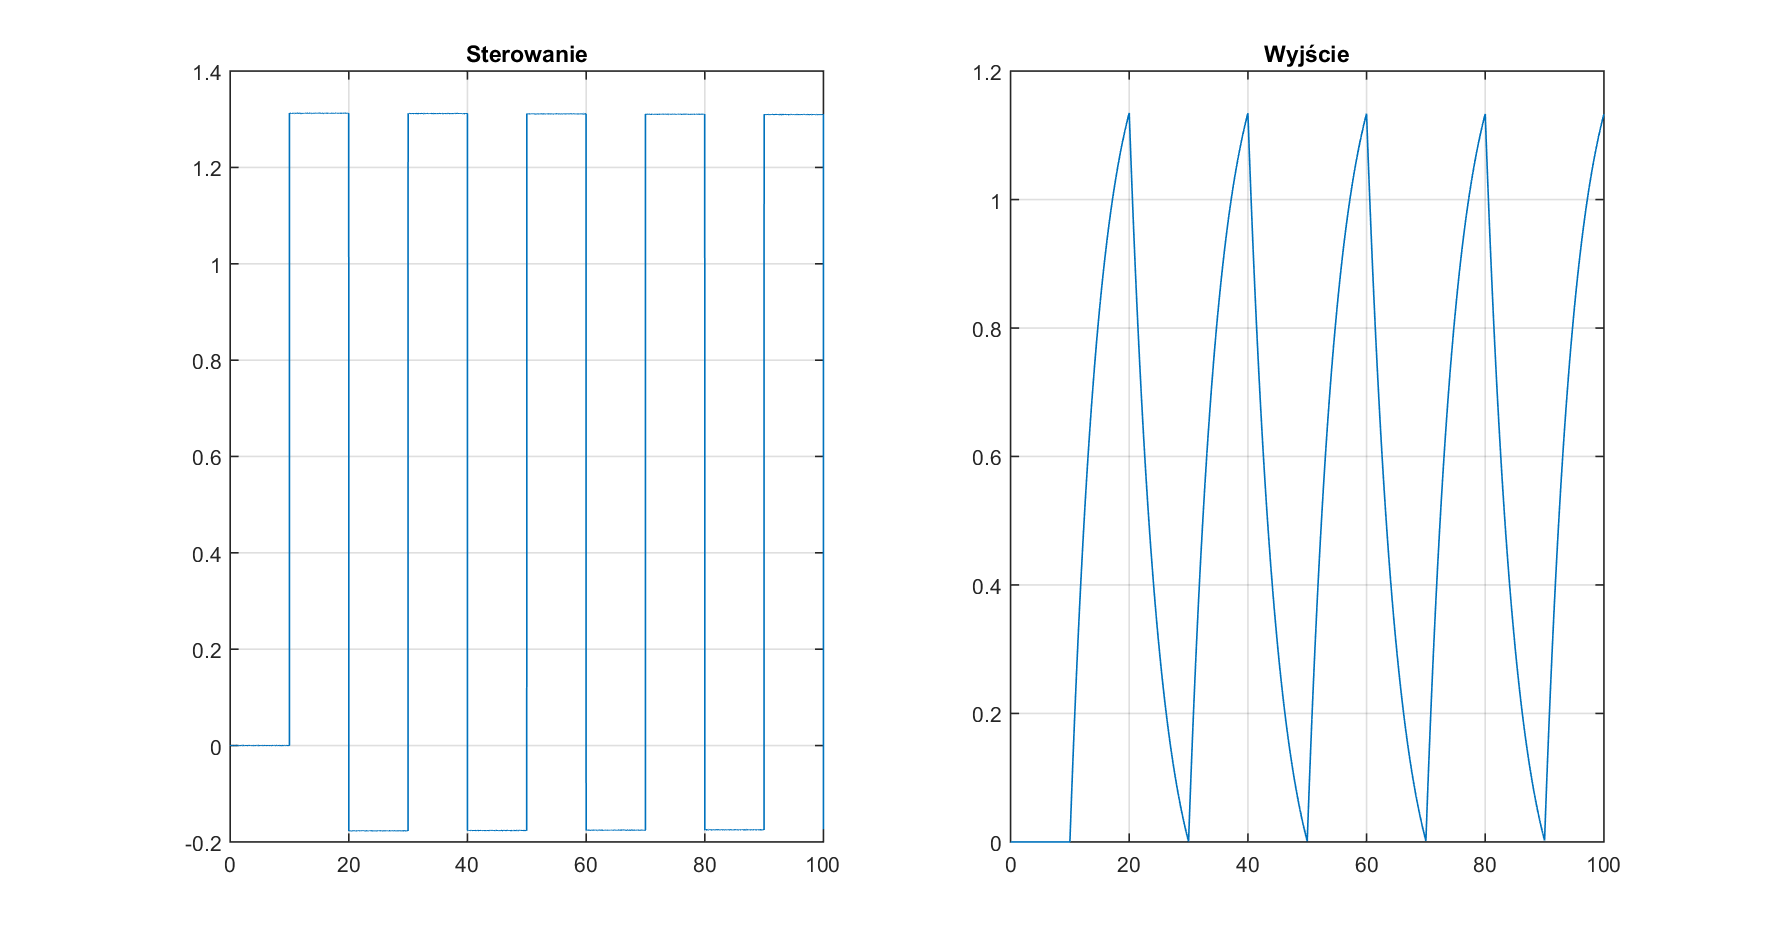
\includegraphics[width = \textwidth]{./img/jedno_k_1_3125.png}
			\end{figure}
			\noindent Wyniki dla czasu próbkowania $T_p = 5 \, \mathrm{s}$. Wzmocnienie krytyczne $k_{kr} = 2,1625$.
			\begin{figure}[H]
				\centering
				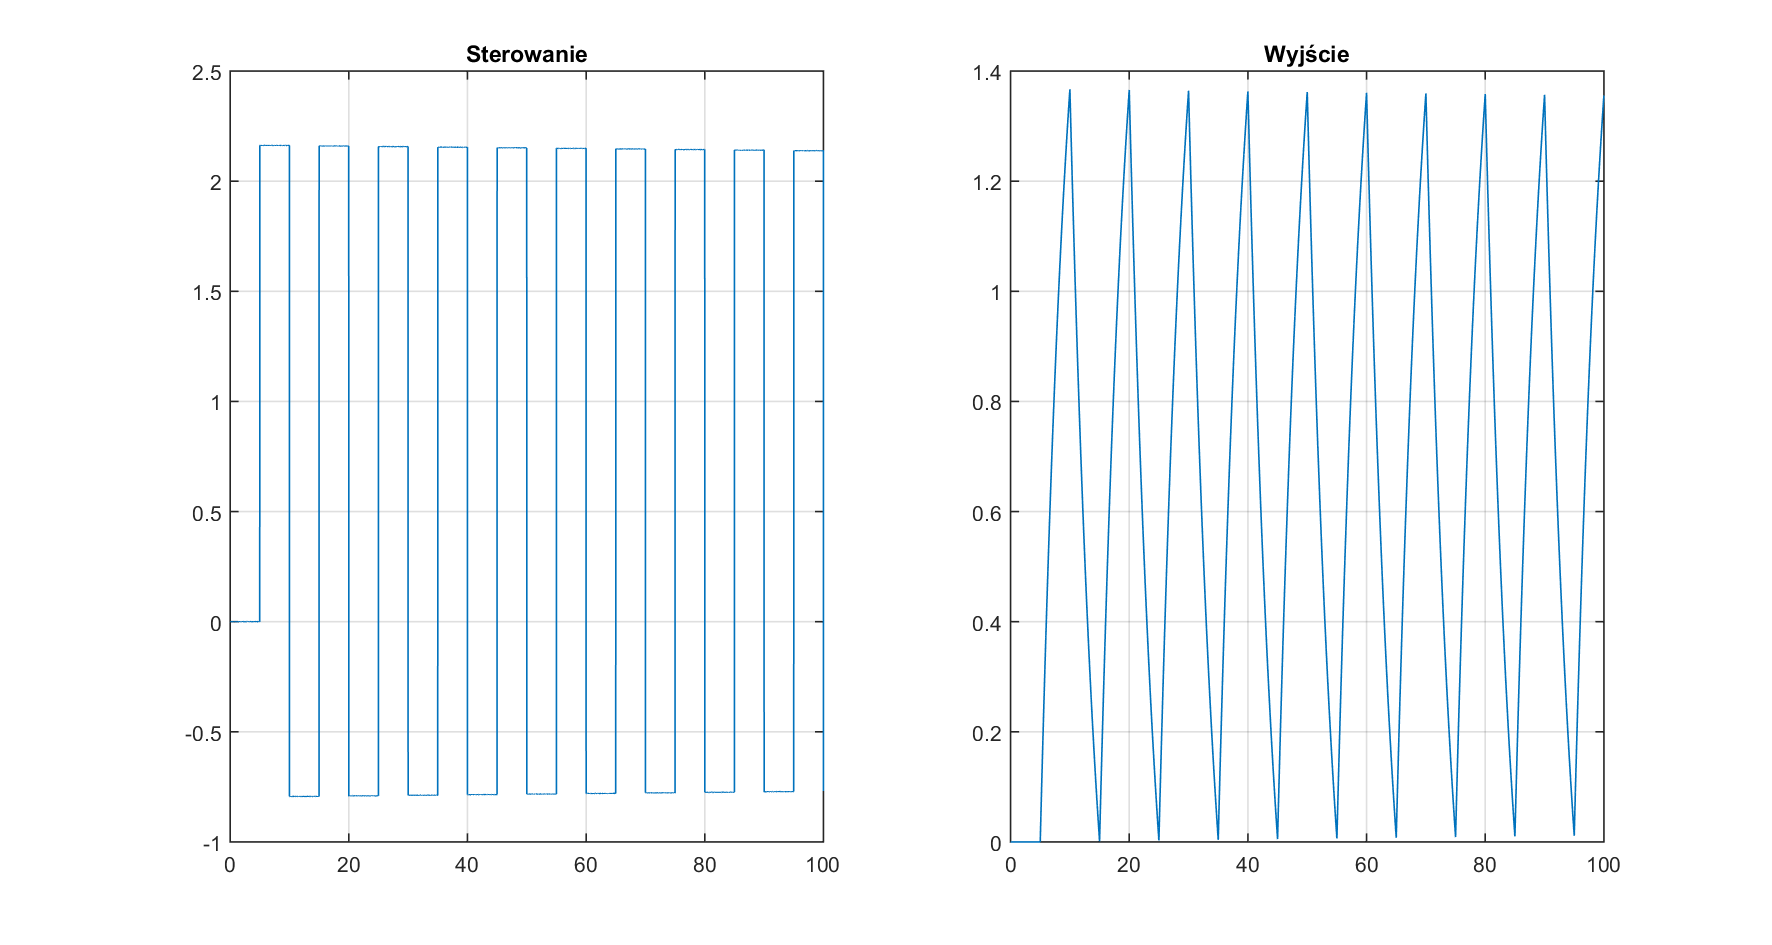
\includegraphics[width = \textwidth]{./img/jedno_k_2_1625.png}
			\end{figure}
			\newpage
			\noindent Wyniki dla czasu próbkowania $T_p = 1 \, \mathrm{s}$. Wzmocnienie krytyczne $k_{kr} = 10,032$.
			\begin{figure}[H]
				\centering
				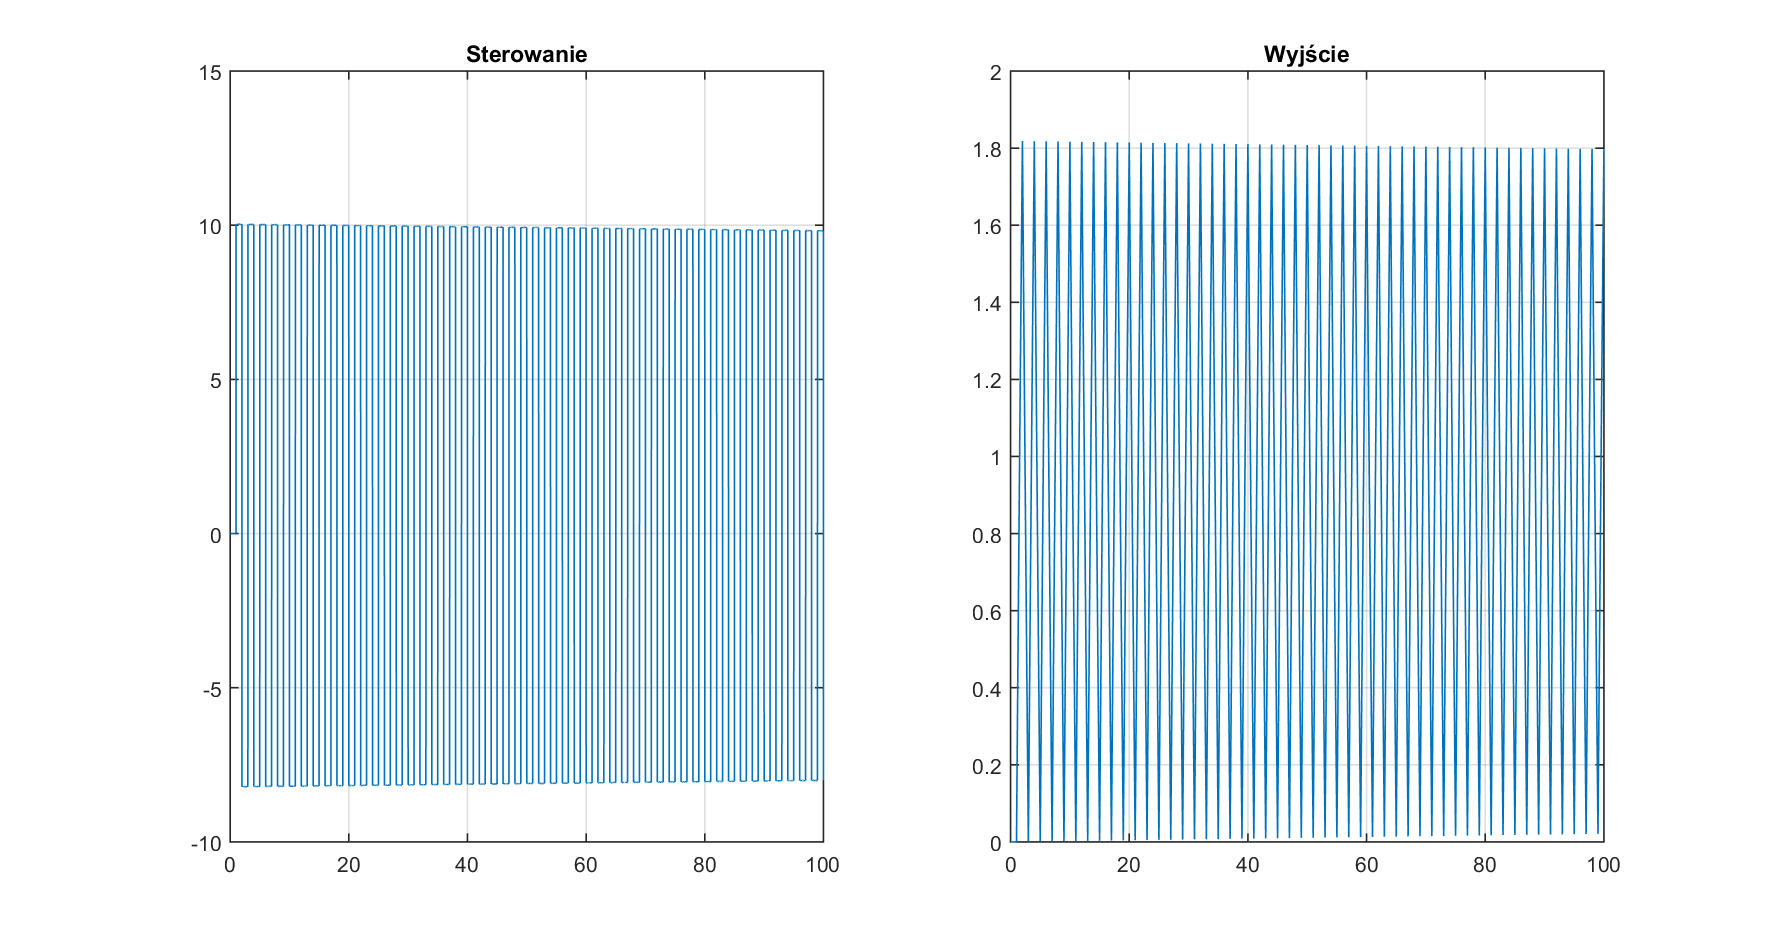
\includegraphics[width = \textwidth]{./img/jedno_k_10_032.png}
			\end{figure}
			\noindent Wyniki dla czasu próbkowania $T_p = 0.1 \, \mathrm{s}$. Wzmocnienie krytyczne $k_{kr} = 100,003$.
			\begin{figure}[H]
				\centering
				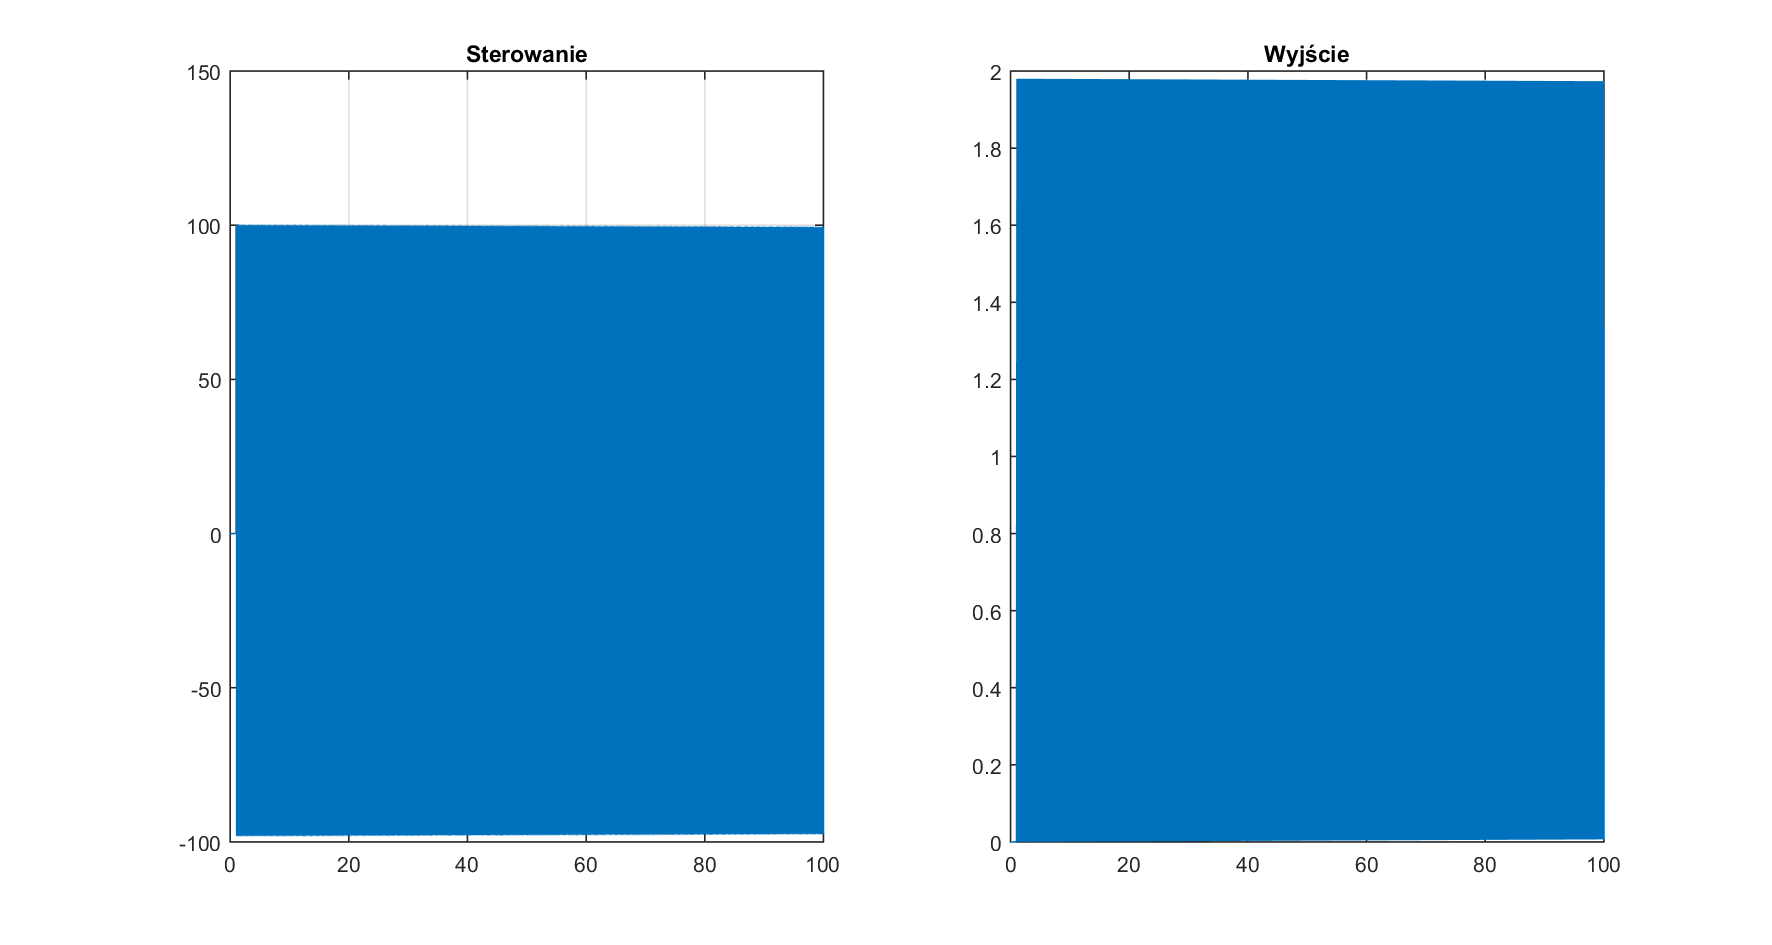
\includegraphics[width = \textwidth]{./img/jedno_k_100_003.png}
			\end{figure}
			\newpage \noindent
			Wyniki dla czasu próbkowania $T_p = 0.01 \, \mathrm{s}$. Wzmocnienie krytyczne $k_{kr} = 1000,0001$.
			\begin{figure}[H]
				\centering
				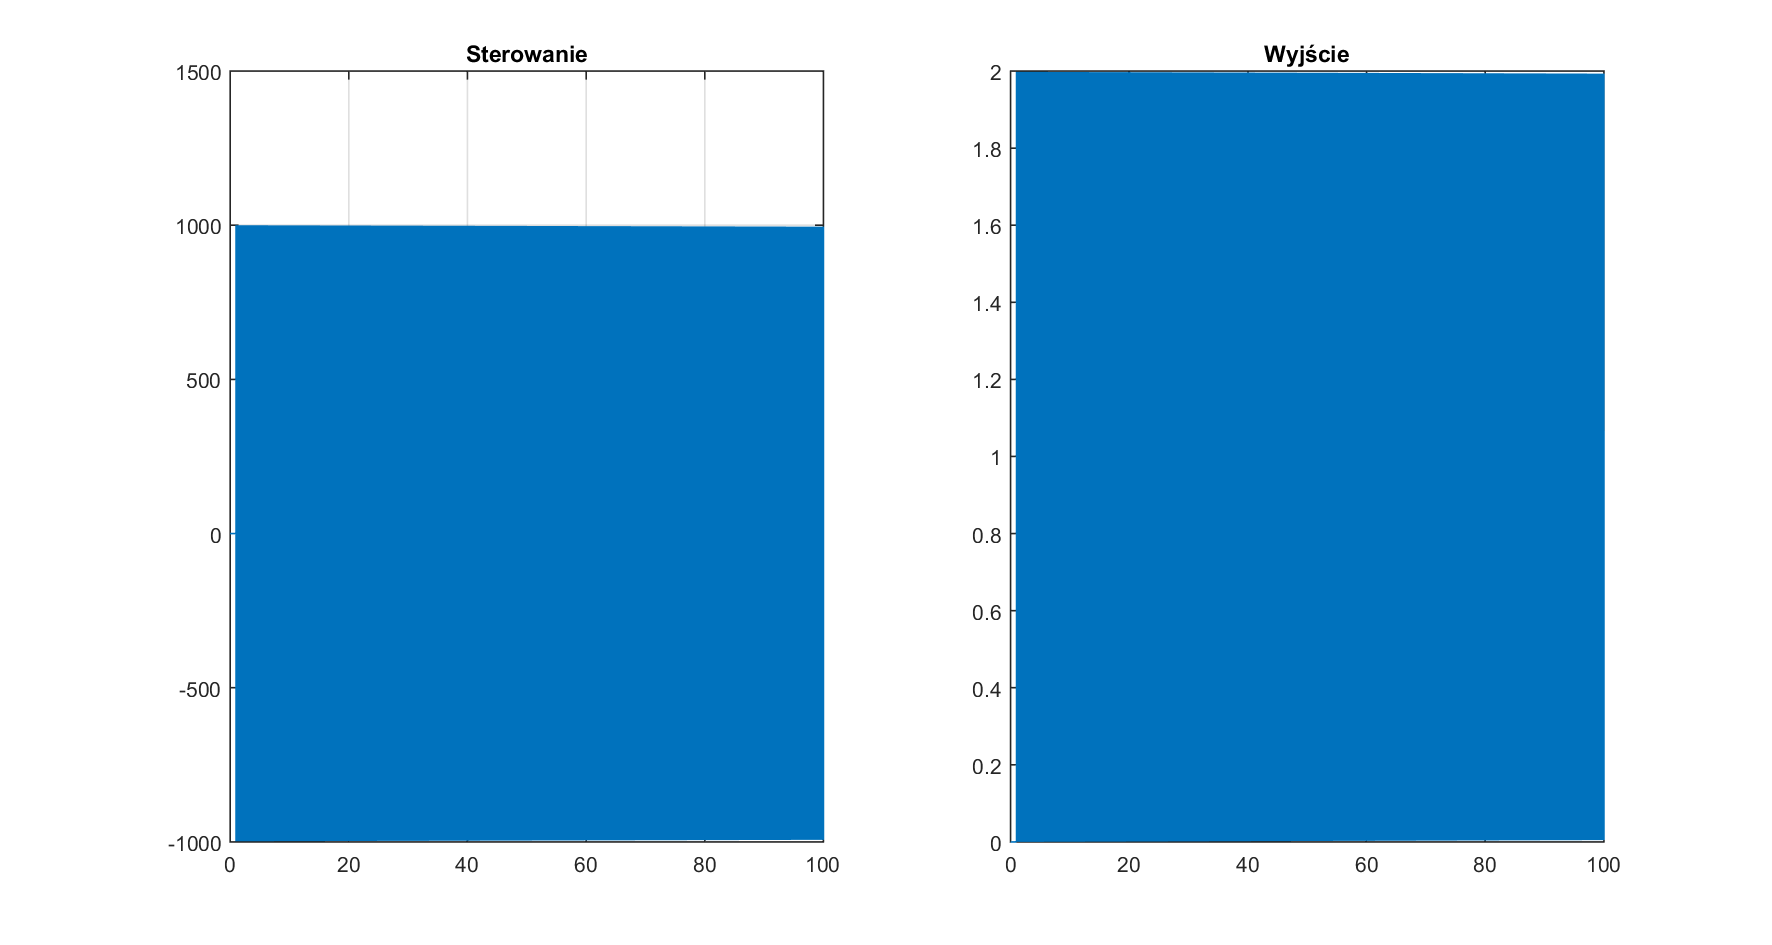
\includegraphics[width = \textwidth]{./img/jedno_k_1000_0001.png}
			\end{figure}
		\subsection{Obiekt inercyjny III rzędu}
			Wyniki dla czasu próbkowania $T_p = 10 \, \mathrm{s}$. Wzmocnienie krytyczne: $k_{kr} = 3,165$.
			\begin{figure}[H]
				\centering
				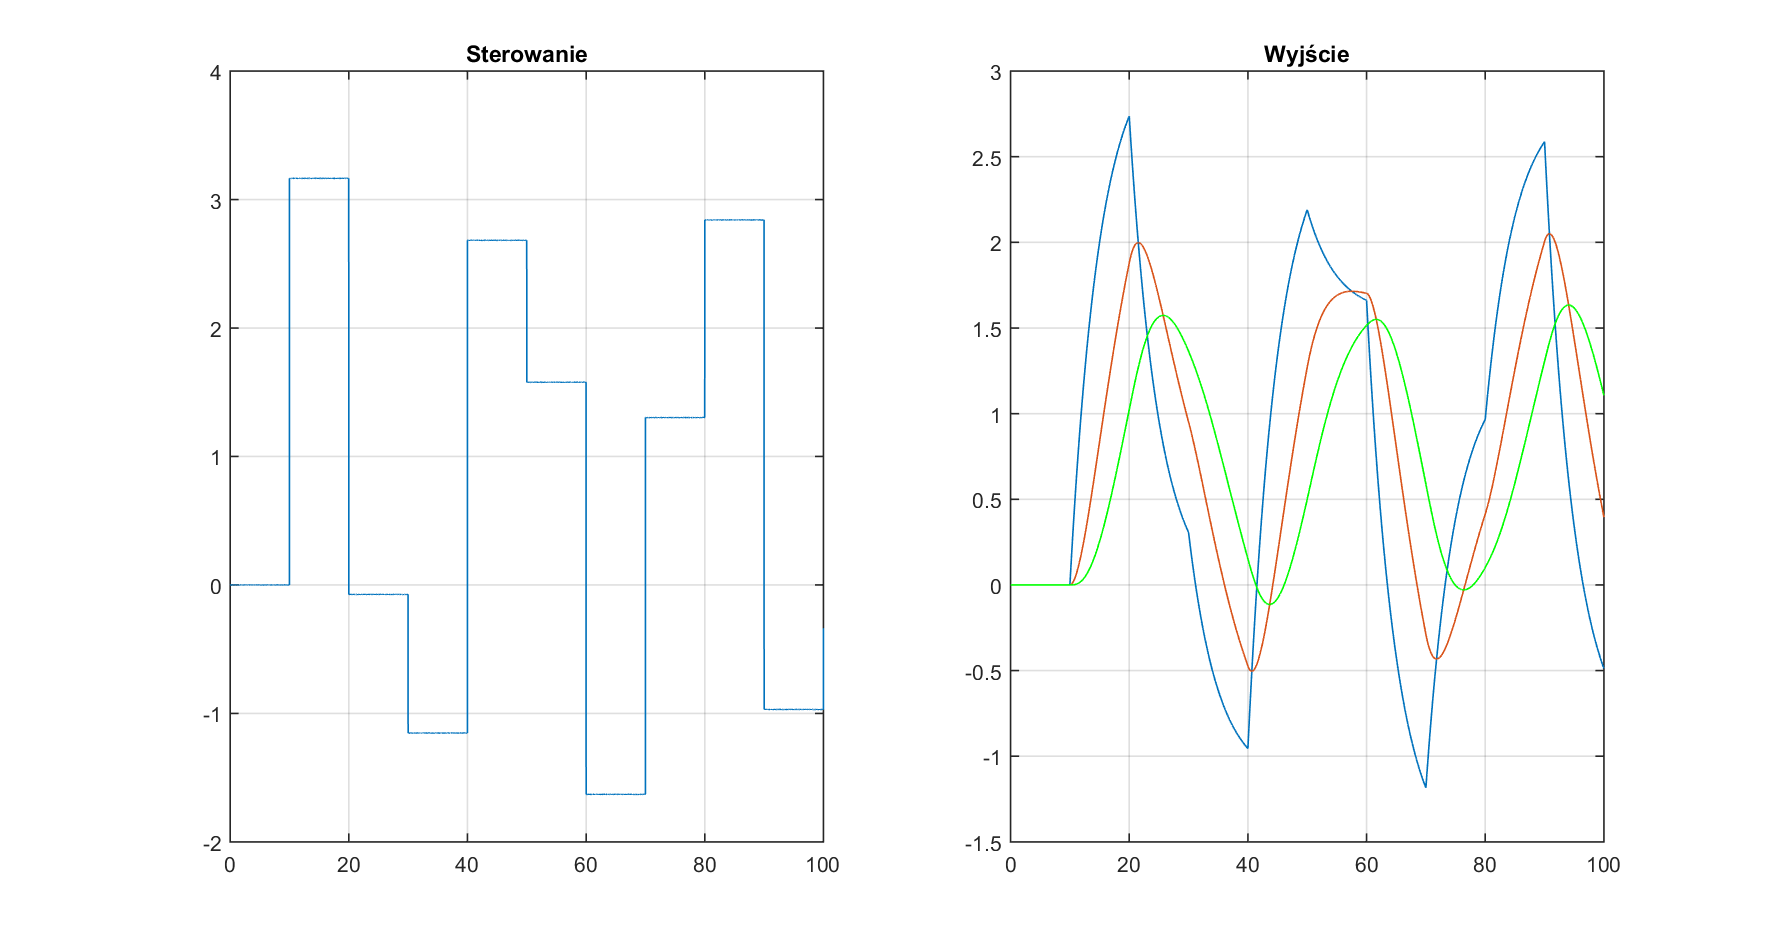
\includegraphics[width = \textwidth]{./img/trzy_k_3_165.png}
			\end{figure}
			\newpage
			\noindent Wyniki dla czasu próbkowania $T_p = 5 \, \mathrm{s}$. Wzmocnienie krytyczne $k_{kr} = 3,75$.
			\begin{figure}[H]
				\centering
				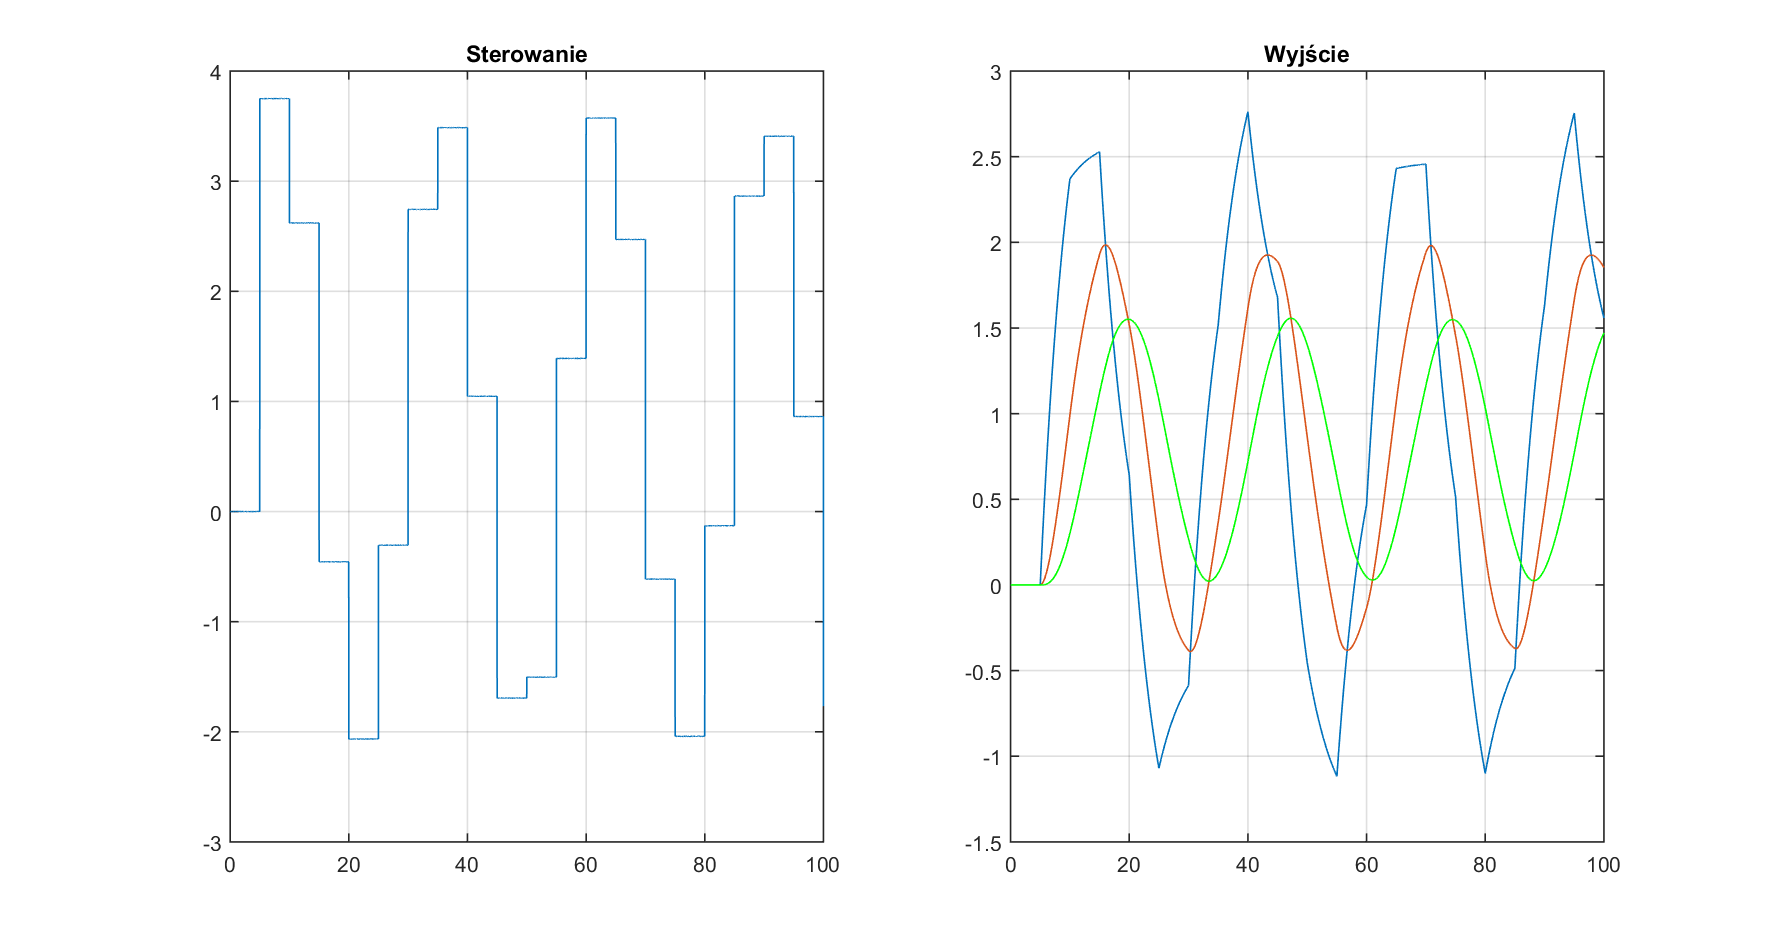
\includegraphics[width = \textwidth]{./img/trzy_k_3_75.png}
			\end{figure}
			\noindent Wyniki dla czasu próbkowania $T_p = 1 \, \mathrm{s}$. Wzmocnienie krytyczne $k_{kr} = 6,25$.
			\begin{figure}[H]
				\centering
				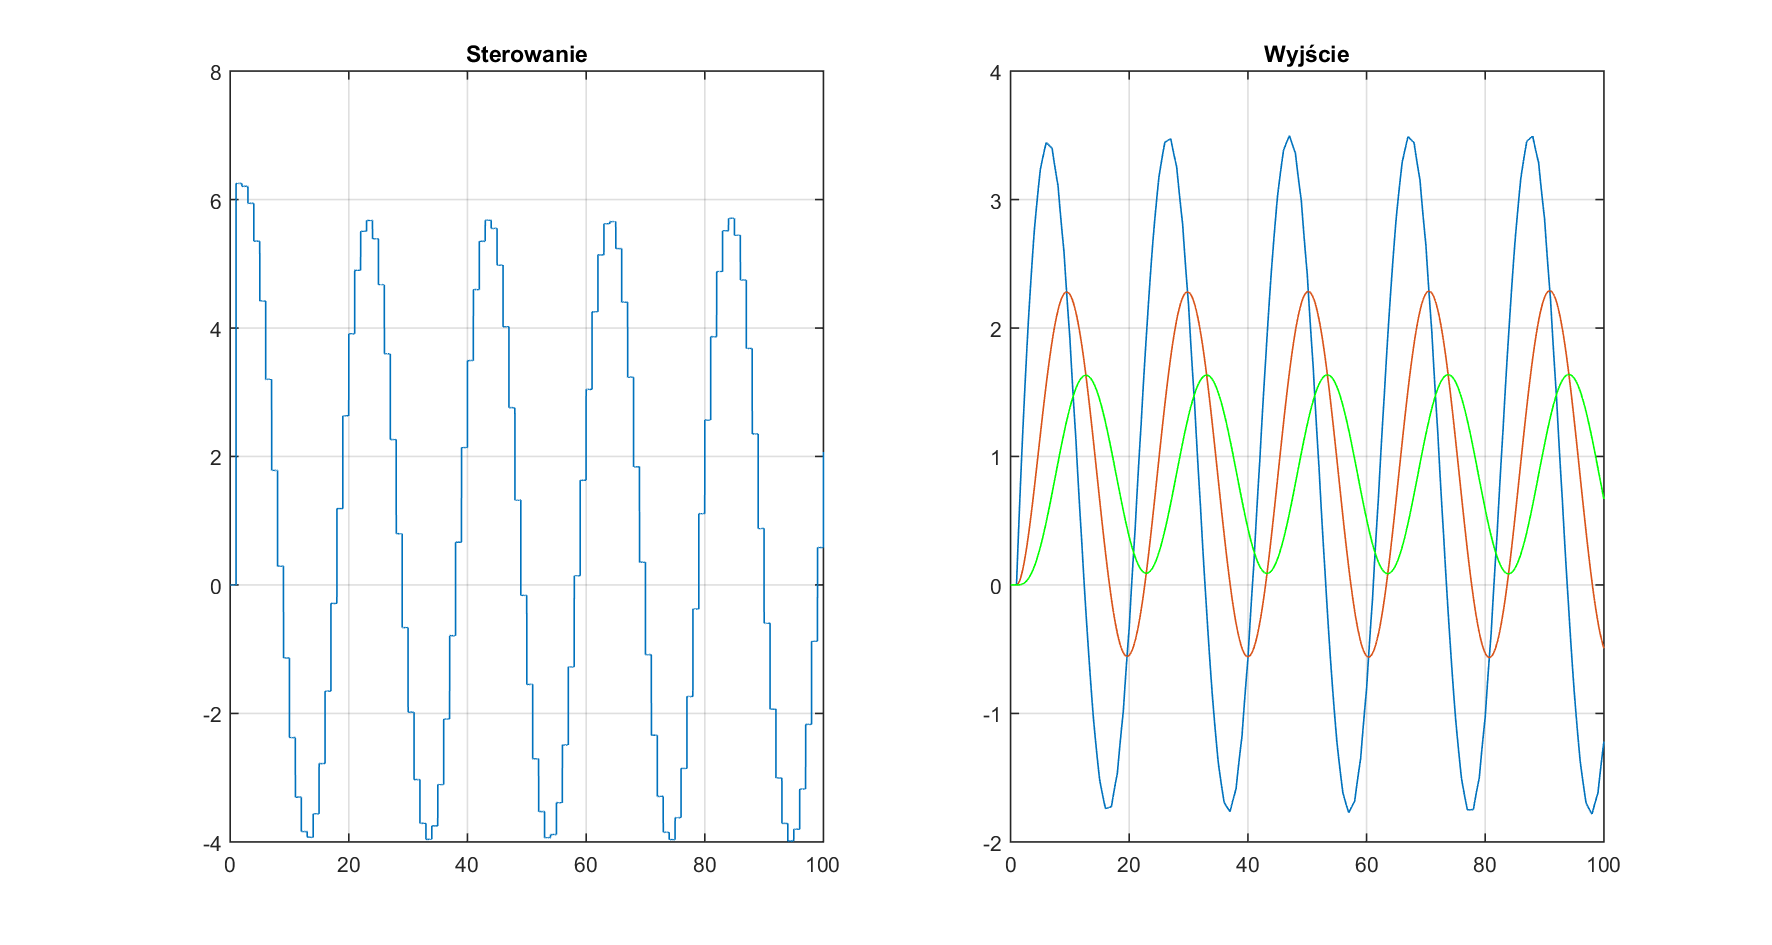
\includegraphics[width = \textwidth]{./img/trzy_k_6_25.png}
			\end{figure}
			\newpage
			\noindent Wyniki dla czasu próbkowania $T_p = 0.1 \, \mathrm{s}$. Wzmocnienie krytyczne $k_{kr} = 7,75$.
			\begin{figure}[H]
				\centering
				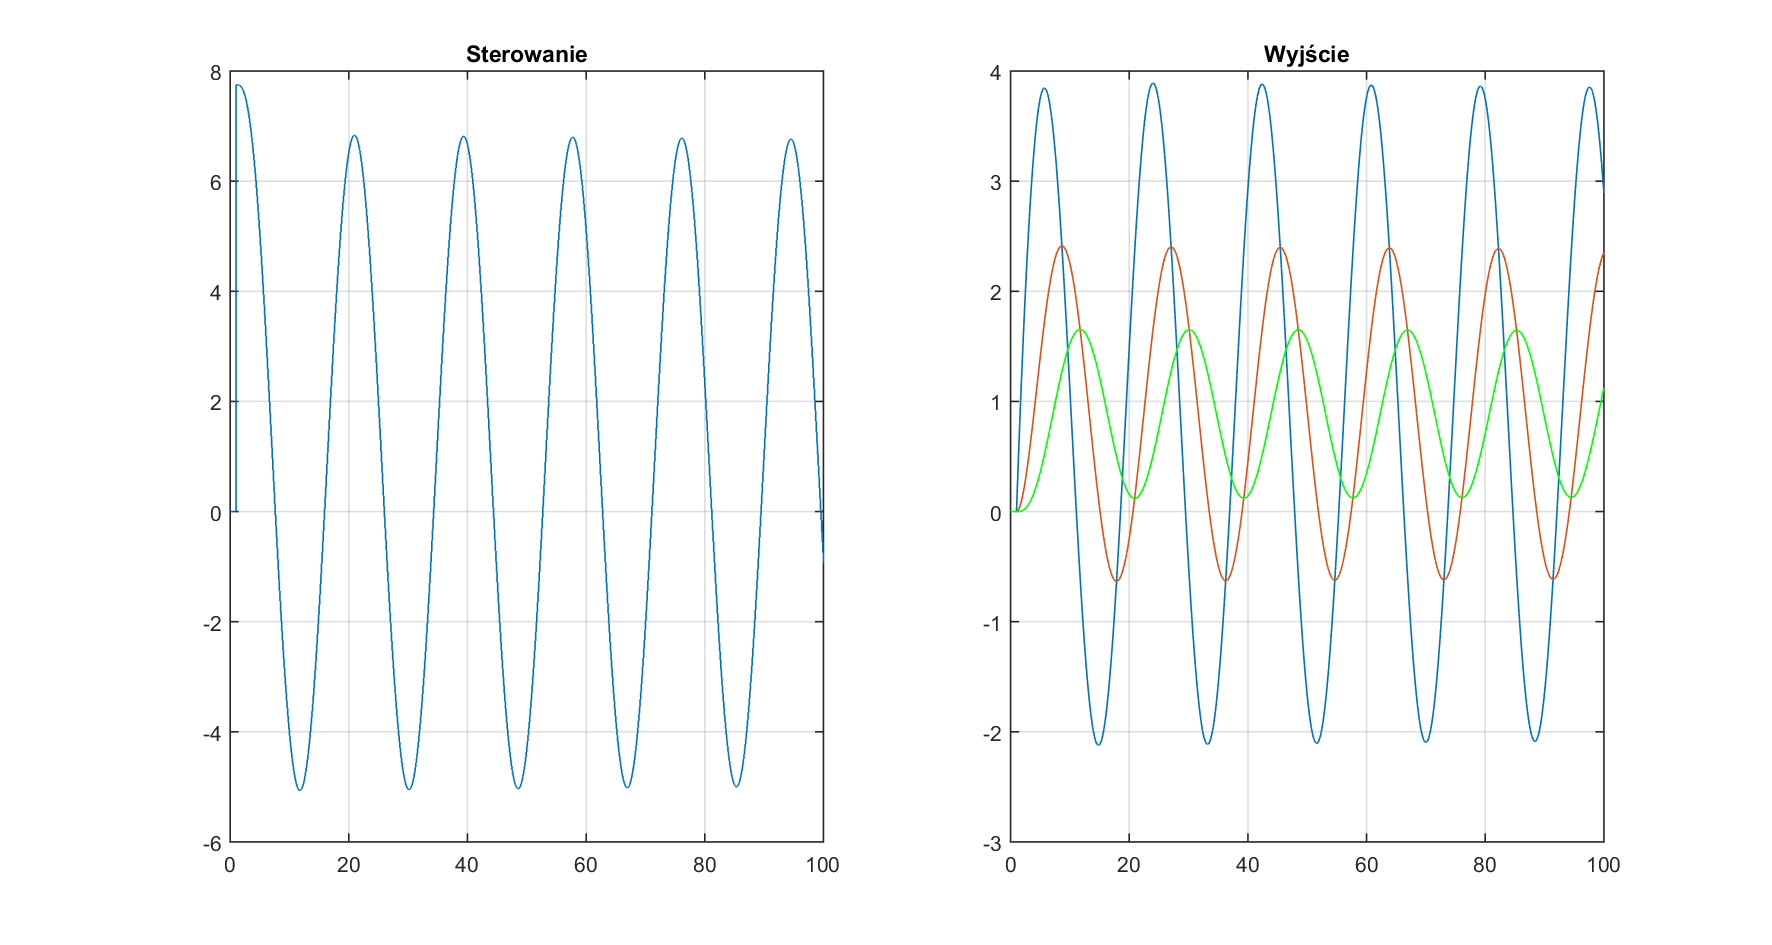
\includegraphics[width = \textwidth]{./img/trzy_k_7_75.png}
			\end{figure}
			\noindent Wyniki dla czasu próbkowania $T_p = 0.01 \, \mathrm{s}$. Wzmocnienie krytyczne $k_{kr} = 7,95$.
			\begin{figure}[H]
				\centering
				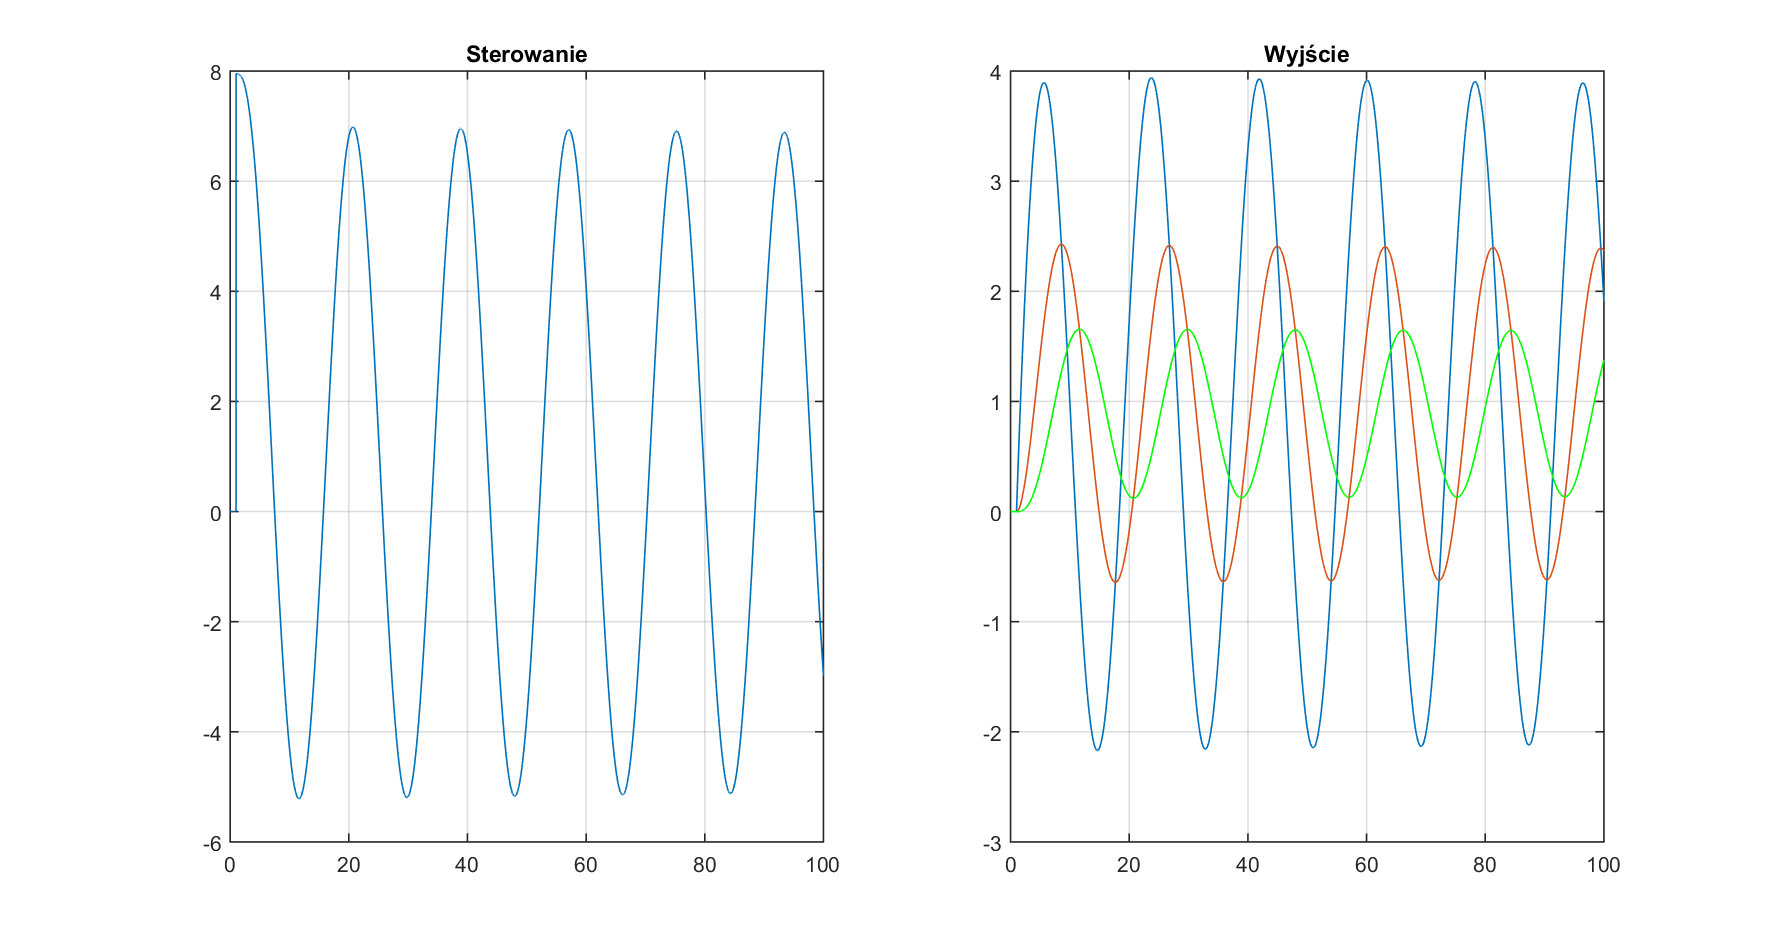
\includegraphics[width = \textwidth]{./img/trzy_k_7_95.png}
			\end{figure}
			\newpage
		\subsection{Wyznaczenie wzmocnienia krytycznego dla układu ciągłego}
			Wzmocnienie krytyczne wyznaczyliśmy tu korzystając z kryterium Nyquista. Ponieważ charakterystyka amplitudowo fazowa obiektu o poniższej transmitancji przecina oś rzeczywistą\linebreak w punkcie (0,125, 0j), to wzmocnienie krytyczne tego układu wynosi $k_{kr} = 8$
			$$
				G(s) = \frac{1}{(5s+1)^3}
			$$
			\begin{figure}[H]
				\centering
				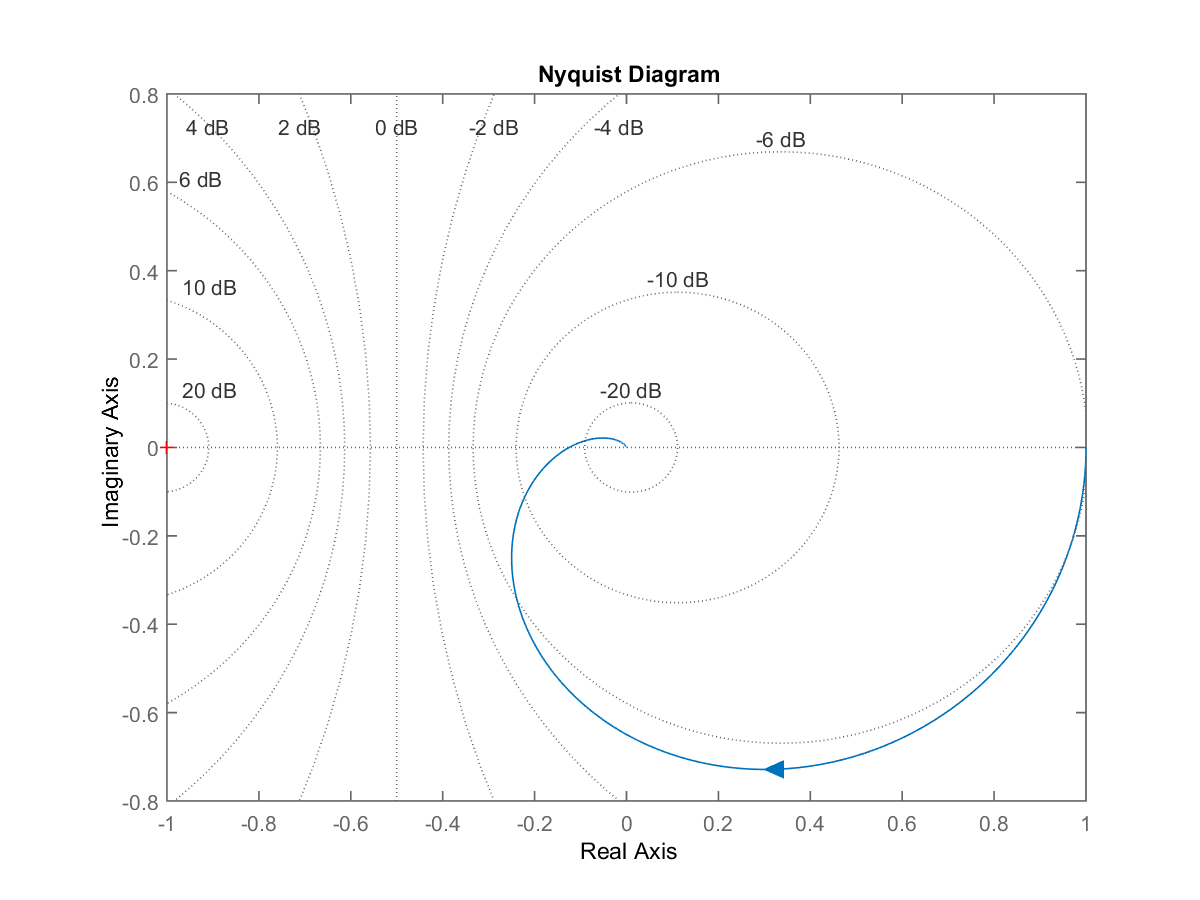
\includegraphics[width = \textwidth]{./img/niquist_k_8.png}
			\end{figure}
	\section{Wnioski}
		Ćwiczenie to pozwoliło nam na zapoznanie się z dyskretnymi układami regulacji. Zapoznaliśmy się na praktycznym przykładzie z ich wadą w stosunku do układów ciągłych -- mogą się zachowywać niestabilnie w przypadkach gdy układy ciągłe są stabilne. Zależy to od okresu próbkowania.
		\newline
		\newline
		Wraz ze wzrostem częstotliwości próbkowania można zauważyć, że wyjście z układu zaczyna się coraz bardziej zachowywać jak dla układu ciągłego, a wzmocnienie krytyczne zbliża się do tego dla układu ciągłego -- dla obiektu inercyjnego I rzędu do nieskończoności, a dla obiektu inercyjnego III rzędu z przykładu do 8.
		\newline 
		\newline
		Mogliśmy również zaobserwować działanie obiektów inercyjnych jako filtru dolnoprzepustowego, poprzez łagodzenie ostrych krawędzi przebiegów. Każdy kolejny człon inercyjny wygładzał coraz bardziej krzywą, nie pozwalając na jej szybkie zmiany (powiązane z dużymi częstotliwościami).
		\newline 
		\newline
		W trakcie wykonywania ćwiczenia natknęliśmy się na trudność ze środowiskiem \linebreak MATLAB/SIMULINK -- nie mogliśmy wyeksportować całego przebiegu z SIMULINKa do MATLABa zza ekstrapolatora. Za każdym razem na około 1000 chwil czasowych było przenoszonych tylko 11 w chwilach czasu, kiedy zmianie uległa wartość. Działo się tak, gdyż oscyloskop SIMULINKowy reaguje na zmianę wartości i tylko te punkty uważa za istotne. Udało nam się jednak ominąć tę trudność dodając do układu, przed oscyloskopem, generator niewielkich liczb pseudolosowych (rzędu $10^{-5}$). Dzięki temu następowały tam niewielkie zmiany, które nie miały wpływu na układ, a nam pozwoliły na wyeksportowanie pełnego zakresu danych, otrzymując przebiegi regulacji składające się z prostokątów, a nie z trapezów.
\end{document}